\documentclass{article}

\usepackage{neurips_2026}

\usepackage[utf8]{inputenc}
\usepackage[T1]{fontenc}
\usepackage{hyperref}
\usepackage{url}
\usepackage{booktabs}
\usepackage{amsmath}
\usepackage{amssymb}
\usepackage{amsthm}
\usepackage{nicefrac}
\usepackage{microtype}
\usepackage{xcolor}
\usepackage{graphicx}

\newtheorem{theorem}{Theorem}
\newtheorem{assumption}{Assumption}
\newtheorem{lemma}{Lemma}

\title{Prediction Defect Equalization for Fast Diffusion Sampling}

\author{%
Wenxin Ge\\
School of Intelligence and Electrical Engineering\\
Huainan Vocational Technical College\\
Huainan, China\\
\And
Jiayu Pan\\
Dept. Software Technology\\
Zhejiang University\\
Hangzhou, China\\
\And
Bingxian Lu\\
School of Computer Science and Engineering\\
Northeastern University\\
Shenyang, China\\
\And
Tie Qiu\\
College of Intelligence and Computing\\
Tianjin University\\
Tianjin, China\\
}

\begin{document}

\maketitle

\begin{abstract}
Denoising diffusion models generate high-quality images by simulating a
reverse trajectory from noise to data, but this iterative procedure becomes
costly when many denoiser evaluations are required. A central challenge in fast
sampling is therefore to choose a discretization schedule that places a small
computational budget at the most important parts of the reverse trajectory.
Existing schedules are often hand-crafted or optimized using indirect criteria
such as distributional bounds, transport costs, or information increments.
These criteria can produce useful grids, but they do not directly reveal where
a particular numerical solver makes its most consequential local errors along
the denoising path. This paper presents \emph{geometric prediction defect
equalization}, a training-free algorithm for automatically selecting sampling
schedules for deterministic diffusion ODE samplers. Our method uses accurate
teacher trajectories from a pretrained model to estimate where a target solver
locally deviates from the intended trajectory, and then allocates time steps to
equalize these geometric prediction defects. The resulting
schedule is solver-aware, coordinate-covariant, and requires no model
retraining, sampler distillation, or tuning of quality-based objectives. We
show that, under a local power-law defect model, our schedule is asymptotically
minimax-optimal for controlling the maximum local distributional prediction
defect. In validated PNDM/CIFAR-10 Euler 50k-sample runs, ours improves
FID over base, native-coordinate linear, and an authorized project-owned
offline-proxy schedule at NFE 10 and 20 across three seeds. Comparisons to
fixed Karras/EDM-style grids and matched SD1.5/SDXL AYS schedules remain
mixed, highlighting the current limits of defect-based schedule calibration.

\end{abstract}

\section{Introduction}
\label{sec:introduction}

Denoising diffusion models generate images by simulating a reverse trajectory
from noise to data. This simulation is accurate when many denoiser evaluations
are available, but those evaluations dominate sampling cost. Fast sampling
therefore asks a concrete allocation question: given only a small number of
function evaluations, where along the reverse trajectory should they be placed?
The answer is not determined by the solver alone. Even a strong numerical
update can fail if its few steps are spent in the wrong regions of the
denoising path.

Discretization schedules are the mechanism for making this allocation. Linear,
polynomial, log-SNR, and EDM-style schedules are simple, stable, and widely
used \citep{karras2022edm}, but they are usually hand-crafted and reused across
models, solvers, and budgets. Recent work shows that this choice can be
optimized. AYS searches for schedules with a solver-specific Girsanov KL upper
bound \citep{sabour2024ays}. Score-Optimal Diffusion Schedules derive a local
path cost from the work performed by a score-based corrector and choose an
inverse path-length schedule \citep{williams2024scoreoptimal}. Other
optimized-timestep methods minimize discrepancies between ODE teacher
solutions and numerical solver trajectories \citep{xue2024optimizedtimesteps}.
These approaches make clear that schedule selection is a central component of
fast diffusion sampling.

However, the criteria used to choose a schedule often remain indirect from the
perspective of the sampler that will actually be run. A distributional bound,
transport-style cost, or path information increment can justify an effective
grid. These criteria leave open the diagnostic question we care about: where
does this numerical solver make its largest local prediction errors along the
denoising trajectory? Without that information, schedule selection still looks
like global search instead of targeted correction of the solver's failure modes.

We present \emph{geometric prediction defect equalization}, a training-free
algorithm for automatically selecting schedules for deterministic diffusion ODE
samplers. Our method uses accurate teacher trajectories from a pretrained model
to estimate where a target student solver locally deviates
from the intended trajectory. It then allocates time steps so that these local
geometric prediction defects are equalized across the schedule.

The details of our method are designed to make this diagnostic meaningful. Each
defect probe starts from the correct teacher state, so it measures one-step
solver error rather than error accumulated from previous approximate steps.
Teacher trajectories are treated as Monte Carlo samples from the teacher
marginal at each noise level, so the estimated defect profile is
distributional rather than path-specific. A state-space metric and optional
tangent downweighting turn endpoint residuals into geometric prediction
defects. Finally, a local power-law model determines how to convert these
defects into a monitor density whose inverse CDF yields the schedule.

Our contributions are as follows.
\begin{enumerate}
  \item \textbf{A solver-facing schedule objective.} We formulate low-NFE
  schedule selection as distributional local prediction-defect equalization for
  a fixed pretrained model and deterministic sampler.
  \item \textbf{A training-free calibration algorithm.} We estimate local
  oracle-start defects from teacher trajectories, aggregate them over the
  teacher marginal with mean, CVaR, or mixed risk, and construct the schedule
  by inverse-CDF equalization of the induced monitor.
  \item \textbf{Geometry and theory.} We derive the monitor
  $\omega_{\mathcal R}(u)=(\bar a_{\mathcal R}(u)+\epsilon_a)^{1/q}$ from a
  local power-law defect model, prove coordinate covariance of the monitor
  one-form, and prove asymptotic minimax optimality of the inverse-CDF schedule
  for local distributional risk.
  \item \textbf{Scoped empirical evidence.} We report a real PNDM/CIFAR-10
  smoke gate, three-seed 50k CIFAR-10 FID results including base, linear,
  Karras-style fixed, and authorized project-owned offline-proxy schedules,
  matched SD1.5 and SDXL CFG sweeps retained as text-to-image boundary
  evidence, and model-evaluation-equivalent calibration cost accounting.
\end{enumerate}

The empirical claims are deliberately bounded. On PNDM/CIFAR-10 with the Euler
solver, our schedule improves FID over base, native-coordinate linear, and the
project-owned offline-proxy schedule at NFE 10 and 20. The comparison to a
fixed Karras/EDM-style grid is mixed: ours wins at NFE 10 and trails
slightly at NFE 20. The matched text-to-image sweeps show condition-dependent
behavior: SD1.5 is negative under these metrics, while SDXL improves
ImageReward against base at CFG 5.0 and 7.5 and has positive mean deltas
against AYS at CFG 7.5. We therefore present our method as a way to expose and
equalize solver-local
trajectory defects; direct optimization of FID, CLIPScore, ImageReward, or
human preference remains outside the claim.

\section{Related Work}
\label{sec:related-work}

Our method sits between schedule optimization and solver design. The closest
prior work asks how to choose the discretization grid; our distinction is that
we estimate the local oracle-start defect of the target solver under the
teacher marginal and then convert that defect into an equal-mass monitor.

\textbf{Diffusion samplers and hand-designed schedules.}
DDPMs, DDIMs, and score-SDE samplers define reverse generative dynamics and
expose a finite set of model-evaluation locations
\citep{ho2020ddpm,song2022ddim,song2021sde}. EDM makes the design space of
preconditioning, noise parameterization, and polynomial noise schedules explicit
\citep{karras2022edm}. These schedules are cheap, stable, and reusable, which
makes them strong practical baselines. They are not, however, diagnostics of a
particular solver's local prediction defect.

\textbf{Offline and path-geometric schedule optimization.}
AYS is the strongest direct schedule-optimization baseline in our setting. It
uses stochastic calculus to build a Girsanov-based KL upper bound between the
true generative SDE and a solver-induced linearized SDE, then searches for a
schedule specific to a model, dataset, and solver \citep{sabour2024ays}. Its
published Stable Diffusion schedules are therefore important baselines in the
text-to-image sweep.

Score-Optimal Diffusion Schedules are especially close conceptually
\citep{williams2024scoreoptimal}. Williams et al. define a diffusion path cost
from the work a Langevin corrector must perform after a predictor step. The
resulting optimal generator is an inverse path-length parameterization: local
costs are equalized along the sampling path. We keep this equalization
principle but change the object being equalized. Instead of a path-intrinsic
score-corrector cost under perfect-score assumptions, we measure the
oracle-start one-step residual of the actual deterministic solver against a
teacher flow, aggregate it over $p_u$, and use the $q$-th root dictated by the
measured local defect order.

Other optimized-timestep methods also move beyond fixed grids. Xue et al.
optimize time steps by minimizing the distance between a ground-truth ODE
solution and the numerical solution induced by a specific solver
\citep{xue2024optimizedtimesteps}. This is close to the teacher-student
motivation of our method, but their method solves an offline constrained
optimization problem, whereas ours estimates a distributional local defect
profile and materializes the schedule by inverse-CDF equalization.

\textbf{Solver acceleration.}
PNDM, DPM-Solver, DPM-Solver++, UniPC, and related predictor-corrector solvers
reduce sampling cost by changing the numerical update rule
\citep{liu2022pndm,lu2022dpmsolver,lu2025dpmsolverpp,zhao2023unipc}. STORK
uses stabilized Taylor orthogonal Runge--Kutta ideas to improve mid-NFE
diffusion and flow-matching sampling while addressing stiffness and
structure-dependence \citep{tan2025stork}. These methods are complementary to
our method: they change how a step is computed, while ours changes where a
fixed solver evaluates the model. The distinction also matters for theory. Our
main guarantee is stated for deterministic oracle-start ODE defects; multistep,
stochastic, and scheduler-history solvers require either augmented-state
analysis or empirical framing.

\textbf{Learned fast samplers.}
Differentiable sampler search and progressive distillation reduce NFE by
optimizing sampler parameters or distilling many-step samplers into fewer-step
generators \citep{watson2022fastsamplers,salimans2022progressive}. Our method
does not update model weights and does not optimize an image-quality objective.
Negative cases therefore diagnose the schedule monitor and its calibration
distribution rather than a learned generator.

\section{Method}
\label{sec:method}

Our method turns the practical question of low-NFE sampling into a calibration
problem. The input is a pretrained diffusion model, a deterministic sampler
that will be used at inference, and a desired number of steps. The output is a
schedule that spends more of those steps where the sampler's own one-step
prediction is locally unreliable. This section first defines the teacher and
student objects, then shows how teacher trajectories are used to estimate a
defect monitor and invert it into a schedule.

\subsection{Problem setup}

We start from a deterministic diffusion or flow ODE written in a
monotone sampling coordinate $u$:
\begin{equation}
  \frac{dx}{du}=f_\theta(x,u),
  \qquad u\in[u_{\min},u_{\max}].
  \label{eq:ode}
\end{equation}
The coordinate may denote time, noise level, log-SNR, or another smooth
monotone reparameterization. Let $F_{a\rightarrow b}(x)$ denote the exact
teacher flow, approximated in practice by high-accuracy numerical integration
of Eq.~\eqref{eq:ode}. If $x_0\sim p_{u_{\min}}$, the teacher marginal at
coordinate $u$ is the pushforward
\begin{equation}
  p_u=(F_{u_{\min}\rightarrow u})_{\#}p_{u_{\min}}.
  \label{eq:teacher-marginal}
\end{equation}
A fixed student solver $\mathcal S$ performs a one-step update
$\Phi_{\mathcal S}(x;u\rightarrow v)$ that approximates
$F_{u\rightarrow v}(x)$. Given a target number of steps $N$, the goal is to
construct a schedule
\begin{equation}
  U=(u_0<u_1<\cdots<u_N),\qquad
  u_0=u_{\min},\quad u_N=u_{\max},
\end{equation}
without retraining $f_\theta$ or changing the solver.

\begin{figure}[t]
  \centering
  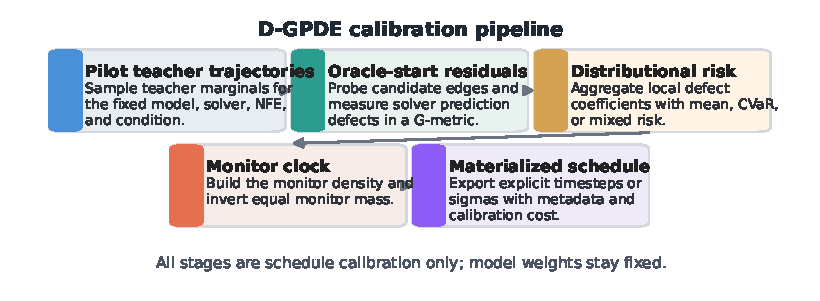
\includegraphics[width=\linewidth]{figures/dgpde_method_overview.pdf}
  \caption{Our calibration pipeline. Teacher trajectories define
  oracle-start residual probes, distributional risk forms a monitor clock, and
  equal-monitor-mass inversion materializes a solver-aware schedule. The
  schematic contains method structure only.}
  \label{fig:method-overview}
\end{figure}

\subsection{Teacher trajectories sample teacher marginals}

We draw $K$ calibration initial states $x_{k,0}\sim p_{u_{\min}}$ and compute
high-accuracy teacher trajectories
\begin{equation}
  x_k^\star(u)=F_{u_{\min}\rightarrow u}(x_{k,0}),
  \qquad k=1,\ldots,K.
\end{equation}
By Eq.~\eqref{eq:teacher-marginal}, for every coordinate $u$ the set
$\{x_k^\star(u)\}_{k=1}^K$ is a Monte Carlo sample from $p_u$. Calibration
therefore estimates a distributional object: the local state distribution on
which the student solver is evaluated.

\subsection{Geometric oracle-start defect}

We evaluate endpoint residuals with a positive definite state-space metric
$G(u)\succ0$:
\begin{equation}
  \langle r_1,r_2\rangle_{G(u)}=r_1^\top G(u)r_2,
  \qquad
  \|r\|_{G(u)}^2=r^\top G(u)r .
\end{equation}
The metric can normalize errors across noise levels, channels, or latent-space
scalings; examples include isotropic noise normalization
$G(u)=(\sigma(u)^2+\sigma_{\rm data}^2)^{-1}I$ or channel-wise whitening.

For trajectory $k$, define the $G$-unit teacher tangent
\begin{equation}
  T_{k,G}(u)
  =
  \frac{\partial_u x_k^\star(u)}
  {\|\partial_u x_k^\star(u)\|_{G(u)}}
  =
  \frac{f_\theta(x_k^\star(u),u)}
  {\|f_\theta(x_k^\star(u),u)\|_{G(u)}}.
\end{equation}
When the tangent norm is numerically unstable, we use the full residual by
setting $\rho=1$. For a residual $r$ measured at endpoint $b$, define
\begin{equation}
  \|r\|_{\rho,k,b}^2
  =
  r^\top G(b)r
  -(1-\rho)\left(T_{k,G}(b)^\top G(b)r\right)^2,
  \qquad \rho\in(0,1].
  \label{eq:mixed-norm}
\end{equation}
Equivalently, if $r=r_\parallel^{G(b)}+r_\perp^{G(b)}$ is the
$G(b)$-orthogonal tangent-normal decomposition, then
\begin{equation}
  \|r\|_{\rho,k,b}^2
  =
  \|r_\perp^{G(b)}\|_{G(b)}^2
  +
  \rho\|r_\parallel^{G(b)}\|_{G(b)}^2.
  \label{eq:mixed-decomposition}
\end{equation}
Thus $\rho=1$ gives the full residual, while $0<\rho<1$ downweights
phase-like tangent error and emphasizes normal deviation from the teacher
trajectory.

For $x\sim p_u$, the oracle-start local prediction defect of the student solver
over $[u,v]$ is
\begin{equation}
  d_{\mathcal S}(x;u,v)
  =
  \left\|
  \Phi_{\mathcal S}(x;u\rightarrow v)-F_{u\rightarrow v}(x)
  \right\|_{\rho,u,v}^{2}.
  \label{eq:oracle-defect-distribution}
\end{equation}
On calibration trajectory $k$, this becomes
\begin{equation}
  d_k(u,v)
  =
  \left\|
  \Phi_{\mathcal S}(x_k^\star(u);u\rightarrow v)-x_k^\star(v)
  \right\|_{\rho,k,v}^{2}.
  \label{eq:oracle-defect-empirical}
\end{equation}
Every measurement starts from $x_k^\star(u)$, not from a student state reached
after previous approximate steps. The defect therefore measures intrinsic
one-step solver error rather than a mixture of local defect and accumulated
prefix error.

\subsection{Local coefficient estimation and risk aggregation}

For small $h>0$, assume the local expansion
\begin{equation}
  d_{\mathcal S}(x;u,u+h)
  =
  a_{\mathcal S}(x,u)h^q+O(h^{q+1}),
  \label{eq:local-power-law-method}
\end{equation}
where $q>0$ is the effective squared-defect order and
$a_{\mathcal S}(x,u)\ge0$ is a local defect coefficient. Along trajectory $k$,
$d_k(u,u+h)=a_k(u)h^q+O(h^{q+1})$ with
$a_k(u)=a_{\mathcal S}(x_k^\star(u),u)$. Given a probe step $\eta$, a
single-probe estimate is
\begin{equation}
  \widehat a_k(u)=\frac{d_k(u,u+\eta)}{\eta^q}.
\end{equation}
When $q$ is unknown, we use multiple probe sizes $\eta_j$ and fit
\begin{equation}
  \log d_k(u,u+\eta_j)\approx \log a_k(u)+q\log\eta_j
\end{equation}
by pooled log-log regression over trajectories and probe grid points.

Let $\mathcal R$ be a risk functional over nonnegative random variables. The
distributional defect coefficient is
\begin{equation}
  \bar a_{\mathcal R}(u)
  =
  \mathcal R_{x\sim p_u}\!\left[a_{\mathcal S}(x,u)\right],
  \label{eq:distributional-a}
\end{equation}
estimated empirically by
\begin{equation}
  \widehat{\bar a}_{\mathcal R}(u)
  =
  \mathcal R_{k=1}^K\!\left[\widehat a_k(u)\right].
\end{equation}
We use mean risk, CVaR risk, or a mean-CVaR mixture:
\begin{align}
  \bar a_{\rm mean}(u)
  &=\frac{1}{K}\sum_{k=1}^K\widehat a_k(u),\\
  \bar a_{\rm CVaR}(u)
  &=\operatorname{CVaR}_{\beta,k}\!\left[\widehat a_k(u)\right],\\
  \bar a_{\alpha,\beta}(u)
  &=(1-\alpha)\bar a_{\rm mean}(u)+\alpha\bar a_{\rm CVaR}(u).
\end{align}
Mean risk targets average teacher-student alignment; CVaR emphasizes
high-error trajectories; the mixture is the default robust choice.

\subsection{Monitor clock and schedule construction}

For a small interval $[u,u+h]$, define the distributional local defect
\begin{equation}
  \bar D_{\mathcal R}(u,u+h)
  =
  \mathcal R_{x\sim p_u}\!\left[d_{\mathcal S}(x;u,u+h)\right].
\end{equation}
The local model implies
$\bar D_{\mathcal R}(u,u+h)=\bar a_{\mathcal R}(u)h^q+O(h^{q+1})$. Equalizing
the leading local risk over intervals with lengths $h_i$ requires
$\bar a_{\mathcal R}(u_i)h_i^q=C$, so the sampling density should be
proportional to $\bar a_{\mathcal R}(u)^{1/q}$. We define the monitor
\begin{equation}
  \omega_{\mathcal R}(u)
  =
  \left(\bar a_{\mathcal R}(u)+\epsilon_a\right)^{1/q},
  \label{eq:monitor}
\end{equation}
where $\epsilon_a>0$ is a numerical floor. Its interval mass is
\begin{equation}
  \mathcal M_{\mathcal R}([a,b])
  =
  \int_a^b\omega_{\mathcal R}(u)\,du.
\end{equation}
Let $\Omega_{\mathcal R}=\int_{u_{\min}}^{u_{\max}}\omega_{\mathcal R}(u)\,du$
and define the normalized monitor clock
\begin{equation}
  \tau_{\mathcal R}(u)
  =
  \frac{\int_{u_{\min}}^u\omega_{\mathcal R}(\xi)d\xi}
  {\int_{u_{\min}}^{u_{\max}}\omega_{\mathcal R}(\xi)d\xi}.
  \label{eq:monitor-clock}
\end{equation}
The final $N$-step schedule is the inverse-CDF discretization
\begin{equation}
  u_m=\tau_{\mathcal R}^{-1}\!\left(\frac{m}{N}\right),
  \qquad m=0,\ldots,N,
  \label{eq:inverse-cdf-schedule}
\end{equation}
which gives every interval equal monitor mass.

\paragraph{Calibration procedure.}
Given calibration samples, the teacher solver, target solver, metric, tangent
weight, risk functional, probe grid, probe sizes, and floor, the procedure:
\begin{enumerate}
  \item computes dense teacher trajectories $x_k^\star(u)$;
  \item evaluates oracle-start defects $d_k(u,u+\eta_j)$ on the probe grid;
  \item estimates $q$ and $a_k(u)$ from single probes or pooled log-log fits;
  \item aggregates $\widehat{\bar a}_{\mathcal R}(u)$ across trajectories;
  \item builds $\widehat\omega_{\mathcal R}(u)$, optionally smooths
  $\log\widehat\omega_{\mathcal R}$, and exports
  $u_m=\widehat\tau_{\mathcal R}^{-1}(m/N)$.
\end{enumerate}
The dominant calibration cost is $O(KMJ\,C_{\mathcal S})$, where
$M$ is the probe-grid size, $J$ is the number of probe sizes, and
$C_{\mathcal S}$ is the cost of one student probe. Changing mean aggregation to
CVaR or a mixture does not require additional model evaluations. The
implementation exports explicit timestep or sigma bundles with solver, NFE,
seed, pilot, cache, and calibration-cost metadata.

\section{Theory}
\label{sec:theory}

Our theory concerns deterministic ODE solvers with oracle-start local
defects. The statement excludes stochastic, ancestral, and history-dependent
solver paths unless they are rewritten as deterministic augmented-state systems.
This section derives the monitor in Eq.~\eqref{eq:monitor}, proves coordinate
covariance, and states the local minimax guarantee.

The result has the same structural shape as path-length equalization in
Score-Optimal Diffusion Schedules \citep{williams2024scoreoptimal}: a local
cost density induces a monitor, and the inverse cumulative monitor yields a
constant-speed traversal in that geometry. The difference is the density. In
Score-Optimal scheduling, the density is derived from score-corrector work along
the diffusion path. Here it is the $q$-th root of a distributional
oracle-start solver-defect coefficient, so the monitor is tied to the target
solver and the teacher marginal distribution used during calibration.

\begin{assumption}[Local power law]
\label{assump:local-power-law}
For $x\sim p_u$, the oracle-start defect satisfies
\begin{equation}
  d_{\mathcal S}(x;u,u+h)
  =
  a_{\mathcal S}(x,u)h^q+R(x,u,h),
\end{equation}
where $q>0$, $a_{\mathcal S}(x,u)\ge0$, and
$|R(x,u,h)|\le C_R(x,u)h^{q+1}$.
\end{assumption}

\begin{assumption}[Risk regularity]
\label{assump:risk-regularity}
The risk functional $\mathcal R$ is monotone, positive homogeneous, and
subadditive on nonnegative random variables, and
$\mathcal R_{x\sim p_u}[C_R(x,u)]<\infty$.
\end{assumption}

Expectation, CVaR, worst-case risk, and nonnegative mixtures of coherent risks
satisfy this assumption.

\begin{theorem}[Distributional local power law]
\label{thm:distributional-power-law}
Under Assumptions~\ref{assump:local-power-law}
and~\ref{assump:risk-regularity},
\begin{equation}
  \bar D_{\mathcal R}(u,u+h)
  =
  \bar a_{\mathcal R}(u)h^q+O(h^{q+1}),
\end{equation}
where
\begin{equation}
  \bar D_{\mathcal R}(u,u+h)
  =
  \mathcal R_{x\sim p_u}
  \!\left[d_{\mathcal S}(x;u,u+h)\right],
  \qquad
  \bar a_{\mathcal R}(u)
  =
  \mathcal R_{x\sim p_u}
  \!\left[a_{\mathcal S}(x,u)\right].
\end{equation}
\end{theorem}

\begin{proof}
For expectation, linearity gives
$\bar D_{\mathbb E}=h^q\mathbb E[a_{\mathcal S}]+\mathbb E[R]$, and the
remainder is bounded by $\mathbb E[C_R]h^{q+1}$. For coherent risks, positive
homogeneity gives $\mathcal R[a_{\mathcal S}h^q]=h^q\mathcal R[a_{\mathcal S}]$,
while monotonicity and subadditivity bound the perturbation by
$\mathcal R[|R|]\le\mathcal R[C_R]h^{q+1}$.
\end{proof}

\begin{theorem}[Correct monitor density]
\label{thm:correct-monitor}
Suppose
\begin{equation}
  \bar D_{\mathcal R}(u,u+h)
  =
  \bar a_{\mathcal R}(u)h^q+O(h^{q+1})
\end{equation}
with $\bar a_{\mathcal R}(u)>0$. The leading-order solution of
\begin{equation}
  \min_{\{h_i\}}\max_i \bar a_{\mathcal R}(u_i)h_i^q,
  \qquad \sum_i h_i=L,
\end{equation}
is obtained by equalizing $\bar a_{\mathcal R}(u_i)h_i^q$ across intervals.
The corresponding continuous monitor density is
\begin{equation}
  \omega_{\mathcal R}(u)=\bar a_{\mathcal R}(u)^{1/q}.
\end{equation}
\end{theorem}

\begin{proof}
At leading order, interval $i$ has risk
$E_i=\bar a_{\mathcal R}(u_i)h_i^q$. If two active intervals have
$E_i>E_j$, decreasing $h_i$ and increasing $h_j$ by a sufficiently small amount
preserves $\sum_i h_i=L$ and decreases the maximum risk. Thus all active
intervals satisfy $\bar a_{\mathcal R}(u_i)h_i^q=C$, so
$h_i=C^{1/q}\bar a_{\mathcal R}(u_i)^{-1/q}$. The local sampling density is
therefore proportional to $\bar a_{\mathcal R}(u)^{1/q}$.
\end{proof}

\begin{theorem}[Coordinate covariance of the monitor]
\label{thm:coordinate-covariance}
Let $v=g(u)$ be a smooth monotone reparameterization. Suppose the same physical
local defect can be expressed as
$\bar D_{\mathcal R}(u,u+h_u)\approx\bar a_u(u)h_u^q$ in $u$-coordinates and
$\bar D_{\mathcal R}(v,v+h_v)\approx\bar a_v(v)h_v^q$ in $v$-coordinates.
Then
\begin{equation}
  \omega_v(v)\,dv=\omega_u(u)\,du,
\end{equation}
where $\omega_u(u)=\bar a_u(u)^{1/q}$ and
$\omega_v(v)=\bar a_v(v)^{1/q}$. Thus $\omega(u)\,du$ is a
coordinate-covariant monitor one-form.
\end{theorem}

\begin{proof}
Small increments satisfy
$h_v=|dv/du|h_u$ and $h_u=|du/dv|h_v$ to leading order. The physical local
defect is invariant under reparameterization, so
$\bar a_u(u)h_u^q=\bar a_v(v)h_v^q$. Substituting
$h_u=|du/dv|h_v$ gives
$\bar a_v(v)=\bar a_u(u)|du/dv|^q$. Taking $q$-th roots yields
$\omega_v(v)=\omega_u(u)|du/dv|$, and multiplication by $dv$ gives the claim.
\end{proof}

\begin{lemma}[Exact equalization of monitor mass]
\label{lem:equal-monitor-mass}
Let $\omega_{\mathcal R}(u)>0$ be continuous on
$[u_{\min},u_{\max}]$, and let
$\Omega_{\mathcal R}=\int_{u_{\min}}^{u_{\max}}\omega_{\mathcal R}(u)du$.
For any $N$-interval schedule, define
$M_i=\int_{u_i}^{u_{i+1}}\omega_{\mathcal R}(u)du$. Then
$\max_i M_i\ge\Omega_{\mathcal R}/N$. Equality holds exactly when all
interval masses are equal, which is achieved by
$u_m=\tau_{\mathcal R}^{-1}(m/N)$.
\end{lemma}

\begin{assumption}[Uniform monitor approximation]
\label{assump:uniform-monitor}
There exists $C_E>0$ such that for all sufficiently small intervals $[s,t]$,
\begin{equation}
  \left|
  \bar D_{\mathcal R}(s,t)-\mathcal M_{\mathcal R}([s,t])^q
  \right|
  \le C_E|t-s|^{q+1}.
\end{equation}
Assume also
$0<\omega_{\min}\le\omega_{\mathcal R}(u)\le\omega_{\max}<\infty$.
\end{assumption}

\begin{theorem}[Asymptotic minimax optimality]
\label{thm:minimax}
Let $U^\Omega$ be the equal-monitor-mass schedule. Under
Assumption~\ref{assump:uniform-monitor},
\begin{equation}
  \max_i\bar D_{\mathcal R}(u_i^\Omega,u_{i+1}^\Omega)
  \le
  \left(\frac{\Omega_{\mathcal R}}{N}\right)^q
  +C_1N^{-(q+1)}.
\end{equation}
Moreover, for any schedule $U$ satisfying $h_{\max}\le C_h/N$,
\begin{equation}
  \max_i\bar D_{\mathcal R}(u_i,u_{i+1})
  \ge
  \left(\frac{\Omega_{\mathcal R}}{N}\right)^q
  -C_2N^{-(q+1)}.
\end{equation}
Thus the equal-monitor schedule is asymptotically minimax optimal for local
distributional risk up to $O(N^{-(q+1)})$.
\end{theorem}

\begin{proof}[Proof sketch]
The equal-mass schedule has monitor mass $\Omega_{\mathcal R}/N$ on every
interval. Since $\omega_{\mathcal R}\ge\omega_{\min}$, its interval lengths are
$O(N^{-1})$, and the upper bound follows from the uniform approximation. For
the lower bound, any schedule has at least one interval with monitor mass at
least $\Omega_{\mathcal R}/N$. If $h_{\max}\le C_h/N$, the approximation error
on that interval is $O(N^{-(q+1)})$. Appendix~\ref{app:minimax-proof} gives the
full proof.
\end{proof}

The implementation uses the regularized monitor
$\omega_\epsilon(u)=(\bar a_{\mathcal R}(u)+\epsilon_a)^{1/q}$ to avoid zero
monitor regions. The same statements apply to the regularized coefficient, and
the unregularized target is recovered as $\epsilon_a\rightarrow0$ on regions
where $\bar a_{\mathcal R}(u)>0$. These results support teacher-oracle local
risk only; perceptual quality and universal FID gains require separate
empirical evidence.

\section{Experiments}
\label{sec:experiments}

Our studies are organized by claim. Final CIFAR-10 claims require
50k generated samples for FID, NFE coverage that includes 10 and 20, and more
than one seed for reliability language, with matched base, native-coordinate
linear, Karras/EDM-style \citep{karras2022edm}, project-owned offline-proxy,
and our schedules. The retained CIFAR backend is PNDM
\citep{liu2022pndm} with the Euler solver. Text-to-image diagnostics require
matched prompt, seed, model, solver, NFE, and guidance-scale keys across base,
published AYS \citep{sabour2024ays}, and our schedules. The repository
also contains STORK adapter tests and scheduler code \citep{tan2025stork}, but
this draft does not report paper-grade STORK quality results.

\begin{table}[t]
  \centering
  \caption{Real PNDM/CIFAR-10 smoke gate for our implementation. The run uses
  Euler, NFE 4, seed 0, and 32 generated samples per
  schedule. FID is reported only to verify that scoring produced finite,
  non-empty outputs; it is not paper-grade evidence.}
  \label{tab:smoke-gate}
  \begin{tabular}{lrrrr}
    \toprule
    Schedule & NFE & Seed & Samples & FID \\
    \midrule
    Base & 4 & 0 & 32 & 295.77 \\
    ours & 4 & 0 & 32 & 258.82 \\
    \bottomrule
  \end{tabular}
\end{table}


Table~\ref{tab:smoke-gate} is a pipeline gate, not a paper result. It verifies
that the repository can materialize our schedule, generate samples for
base and our schedule, compute non-empty FID rows, and write calibration-cost
metadata. The 32-sample FID values cannot support any image-quality claim.

\begin{table}[t]
  \centering
  \caption{PNDM/CIFAR-10 50k FID for the Euler solver. Rows report
  mean $\pm$ standard error over three seeds (0, 1, 2), base, linear
  native-coordinate, fixed Karras/EDM-style, authorized project-owned
  offline, and our schedules. FID is lower-is-better and each
  seed uses 50k generated images. The final two columns are paired
  ours-minus-baseline FID gaps; negative values favor ours.}
  \label{tab:cifar10-pndm-euler-50k-fid-seeds0-1-2}
  {\scriptsize
  \setlength{\tabcolsep}{2pt}
  \resizebox{\linewidth}{!}{%
  \begin{tabular}{rrrrrrrr}
    \toprule
    NFE & base & linear & Karras & offline & ours &
    ours $-$ offline & ours $-$ Karras \\
    \midrule
    10 & 20.57 $\pm$ 0.08 & 20.57 $\pm$ 0.08 & 25.84 $\pm$ 0.10 & 19.20 $\pm$ 0.09 & 17.54 $\pm$ 0.08 & -1.659 $\pm$ 0.017 & -8.302 $\pm$ 0.031 \\
    20 & 11.17 $\pm$ 0.07 & 11.20 $\pm$ 0.07 & 10.64 $\pm$ 0.09 & 10.88 $\pm$ 0.06 & 10.71 $\pm$ 0.07 & -0.175 $\pm$ 0.059 & 0.072 $\pm$ 0.024 \\
    \bottomrule
  \end{tabular}
  }
  }
\end{table}


Table~\ref{tab:cifar10-pndm-euler-50k-fid-seeds0-1-2} records the current
three-seed 50k CIFAR-10 run for NFE 10 and 20, including native-coordinate
linear, fixed Karras/EDM-style, and authorized project-owned offline-proxy
baselines. The offline-proxy rows come from the project-owned coordinate-search optimizer; they
are not published AYS schedules. The result supports only a bounded
controlled-benchmark statement
for the PNDM/CIFAR-10 backend, Euler solver, these two NFE values, and the
reported baseline set. Appendix
Figure~\ref{fig:cifar10-pndm-euler-50k-seeds0-1-2} shows the same aggregate
with per-seed points. Ours improves FID over base, linear, and offline at
both NFE values. The Karras-style grid is worse than ours at NFE 10 but
slightly better at NFE 20, so the positive claim is scoped away from uniform
superiority over fixed schedules. Appendix
Figure~\ref{fig:cifar10-pndm-euler-schedule-profile-nfe20} visualizes the
NFE-20 schedule profiles for seed 0. Appendix
Table~\ref{tab:cifar10-pndm-euler-50k-reuse-seed0-schedule} gives a narrow
actual reuse check for the same backend: reusing the seed-0 schedule
for seeds 1 and 2 has zero observed FID gap because the continuous schedules
round to the same PNDM Euler integer timesteps. Appendix
Tables~\ref{tab:sd15-euler-nfe10-cfg-sweep-pairwise} and
\ref{tab:sdxl-euler-nfe10-cfg-sweep-pairwise} record the matched
text-to-image CFG sweeps where published AYS schedules enter the retained
experiments. SD1.5 is a negative case for our schedule under CLIPScore and
ImageReward. SDXL is condition-dependent: at CFG 5.0 our schedule improves
ImageReward over base but trails AYS, while at CFG 7.5 it improves the mean
CLIPScore and ImageReward deltas against both base and AYS. These sweeps
support CFG-matched coverage and boundary analysis; broad text-to-image
quality improvement remains unsupported. Appendix
Figure~\ref{fig:sd15-euler-nfe10-cfg7p5-schedule-profile} shows the
representative base/AYS/ours sigma-grid diagnostic for CFG 7.5 and seed 0.

\begin{table}[t]
  \centering
  \caption{Calibration cost accounting for current paper-facing runs.
  The quality column reports base-minus-ours FID for CIFAR-10 and
  ours-minus-base ImageReward for text-to-image, so positive values favor
  ours. Model-evaluation equivalents count retained calibration
  cost and the evaluated generation batch, excluding unrelated pilot
  experiments.}
  \label{tab:calibration-cost-summary}
  \begin{tabular}{lllrrr}
    \toprule
    Setting & condition & quality vs. base & cal. evals (M) & gen. evals (M) & cal./gen. \\
    \midrule
    CIFAR-10 & NFE 10 & +3.026 $\pm$ 0.019 FID & 12.73 & 1.500 & 8.49$\times$ \\
    CIFAR-10 & NFE 20 & +0.464 $\pm$ 0.005 FID & 12.73 & 3.000 & 4.24$\times$ \\
    SD1.5 & CFG 5 & -0.133 IR & 25.46 & 0.003 & 8{,}487$\times$ \\
    SD1.5 & CFG 7.5 & -0.084 IR & 25.46 & 0.003 & 8{,}487$\times$ \\
    SD1.5 & CFG 10 & -0.087 IR & 25.46 & 0.003 & 8{,}487$\times$ \\
    SDXL & CFG 5 & +0.079 IR & 0.21 & 0.003 & 68.62$\times$ \\
    SDXL & CFG 7.5 & +0.122 IR & 0.21 & 0.003 & 68.62$\times$ \\
    \bottomrule
  \end{tabular}
\end{table}


Table~\ref{tab:calibration-cost-summary} reports the current calibration-cost
accounting. The CIFAR-10 gain over base comes with calibration cost that exceeds
the evaluated generation batch by 4.24--8.49 times. The SD1.5 sweep has a much
larger calibration-to-generation ratio for the small matched prompt batch and
negative ImageReward deltas. The SDXL rows use a deliberately lighter
calibration configuration and have lower cost ratios, but they still require
schedule reuse across many matched prompt batches for amortization. These
numbers support cost-aware reporting and leave deployment efficiency
unsupported.

\textbf{Takeaway.} The three-seed CIFAR setting improves over base,
native-linear, and authorized project-owned offline-proxy schedules at NFE 10
and 20. The Karras comparison is mixed and stronger at NFE 20. The matched
SD1.5 and SDXL sweeps establish text-to-image coverage, but their automated
metrics are condition-dependent and constrain the claims.

\section{Limitations}
\label{sec:limitations}

Our method equalizes local distributional solver defect rather than final
perceptual quality. It should therefore be interpreted as
teacher-alignment calibration, not as a direct optimizer for FID, CLIPScore,
ImageReward, or human preference. The matched SD1.5 and SDXL CFG sweeps are
retained because they show this distinction concretely.

The minimax result is asymptotic and relies on local power-law behavior. Very
small step counts such as $N=4$ or $N=8$ may fall outside the regime where the
theory is tight. The theory also assumes a deterministic ODE solver with
oracle-start defects; multistep and scheduler-history adapters require an
augmented-state analysis before the theorem applies exactly.

Calibration adds compute before generation. A schedule is practically useful
only when reuse amortizes the teacher and probe cost, so the experiments report
model-evaluation-equivalent calibration cost separately from generation cost.
Finally, the empirical monitor depends on the representativeness of the
calibration trajectories, the teacher solver accuracy, the chosen metric
$G(u)$, and the stability of the fitted order $q$.

\section{Conclusion}

Our method frames low-NFE schedule selection as inference-time distributional
defect equalization. It offers a bounded way to adapt schedules to the
model, solver, NFE, and condition without updating model weights. The theory
supports asymptotic local minimax calibration for deterministic ODE samplers
under a power-law oracle-start defect model. The main positive evidence is the
controlled three-seed CIFAR-10 result against base, native-coordinate linear,
and authorized project-owned offline-proxy schedules, with mixed evidence
against a fixed Karras/EDM-style grid. The matched SD1.5 and SDXL CFG sweeps
identify condition-dependent text-to-image behavior under automated metrics.
A narrow CIFAR reuse check shows no FID penalty when the seed-0 schedule is
reused for seeds 1 and 2 in the same rounded PNDM Euler execution grid. Broader
positive reuse validation, release packaging, and asset-license completion
remain open before submission readiness.


\bibliographystyle{plainnat}
\bibliography{references}

\appendix
\section{Additional Theory Details and Proofs}
\label{app:theory-proofs}

This appendix supplies the proof details that are not central to the main
paper narrative. All results concern oracle-start local defects for
deterministic ODE solvers and support local risk calibration only.

\subsection{Mixed residual decomposition}
\label{app:mixed-residual}

Let $T=T_{k,G}(b)$ satisfy $T^\top G(b)T=1$. The $G(b)$-orthogonal tangent
projection of $r$ is
\begin{equation}
  r_\parallel^{G(b)}=(T^\top G(b)r)T,
\end{equation}
and $r_\perp^{G(b)}=r-r_\parallel^{G(b)}$. Orthogonality gives
\begin{equation}
  \|r\|_{G(b)}^2
  =
  \|r_\perp^{G(b)}\|_{G(b)}^2
  +
  \|r_\parallel^{G(b)}\|_{G(b)}^2,
\end{equation}
with
\begin{equation}
  \|r_\parallel^{G(b)}\|_{G(b)}^2=(T^\top G(b)r)^2.
\end{equation}
Substituting into Eq.~\eqref{eq:mixed-norm} yields
Eq.~\eqref{eq:mixed-decomposition}.

\subsection{Equal monitor mass}
\label{app:equal-monitor-mass}

For completeness we prove Lemma~\ref{lem:equal-monitor-mass}. The interval
masses satisfy $\sum_{i=0}^{N-1}M_i=\Omega_{\mathcal R}$, so their maximum is
at least their average. Equality holds exactly when all masses are equal. Since
$\omega_{\mathcal R}>0$, the cumulative monitor clock
$\tau_{\mathcal R}$ is strictly increasing and invertible, and the inverse-CDF
construction in Eq.~\eqref{eq:inverse-cdf-schedule} gives equal increments of
normalized cumulative mass.

\subsection{Full proof of asymptotic minimax optimality}
\label{app:minimax-proof}

For the equal-mass schedule $U^\Omega$,
\begin{equation}
  \mathcal M_{\mathcal R}([u_i^\Omega,u_{i+1}^\Omega])
  =
  \frac{\Omega_{\mathcal R}}{N}.
\end{equation}
Since $\omega_{\mathcal R}(u)\ge\omega_{\min}$,
\begin{equation}
  h_i^\Omega
  =
  u_{i+1}^\Omega-u_i^\Omega
  \le
  \frac{\Omega_{\mathcal R}/N}{\omega_{\min}}
  =
  O(N^{-1}).
\end{equation}
Using Assumption~\ref{assump:uniform-monitor},
\begin{align}
  \bar D_{\mathcal R}(u_i^\Omega,u_{i+1}^\Omega)
  &\le
  \mathcal M_{\mathcal R}([u_i^\Omega,u_{i+1}^\Omega])^q
  +C_E(h_i^\Omega)^{q+1}\\
  &\le
  \left(\frac{\Omega_{\mathcal R}}{N}\right)^q
  +C_1N^{-(q+1)}.
\end{align}
Taking the maximum over intervals proves the upper bound.

Now consider any admissible schedule $U$ with $h_{\max}\le C_h/N$. Define
$M_i=\mathcal M_{\mathcal R}([u_i,u_{i+1}])$. Since
$\sum_iM_i=\Omega_{\mathcal R}$, there exists $j$ such that
$M_j\ge\Omega_{\mathcal R}/N$. Again by
Assumption~\ref{assump:uniform-monitor},
\begin{align}
  \bar D_{\mathcal R}(u_j,u_{j+1})
  &\ge
  M_j^q-C_Eh_j^{q+1}\\
  &\ge
  \left(\frac{\Omega_{\mathcal R}}{N}\right)^q
  -C_E\left(\frac{C_h}{N}\right)^{q+1}\\
  &=
  \left(\frac{\Omega_{\mathcal R}}{N}\right)^q
  -C_2N^{-(q+1)}.
\end{align}
Therefore the maximum interval defect of any admissible schedule is at least
this lower bound.

\subsection{Monte Carlo estimation of the mean monitor}
\label{app:mc-proof}

Since $x_k^\star(u)\sim p_u$, the random variables
$a_k(u)=a_{\mathcal S}(x_k^\star(u),u)$ are i.i.d. samples from the
distribution of $a_{\mathcal S}(x,u)$ under $p_u$. If the variance is finite,
the central limit theorem gives
\begin{equation}
  \frac{1}{K}\sum_{k=1}^K a_k(u)
  -
  \mathbb E_{x\sim p_u}[a_{\mathcal S}(x,u)]
  =
  O_p(K^{-1/2}).
\end{equation}
If coefficients are estimated from finite probes, write
$\widehat a_k(u)=a_k(u)+\delta_k(u)$ with
$K^{-1}\sum_k\delta_k(u)=O(\varepsilon_{\rm probe}(u))$. Then
\begin{equation}
  \widehat a_{\rm mean}(u)-\bar a_{\rm mean}(u)
  =
  O_p(K^{-1/2})+O(\varepsilon_{\rm probe}(u)).
\end{equation}

\subsection{Inverse-CDF stability}
\label{app:inverse-stability-proof}

Let
\begin{equation}
  F(u)=\int_{u_{\min}}^u\omega_{\mathcal R}(\xi)d\xi,
  \qquad
  \widehat F(u)=\int_{u_{\min}}^u\widehat\omega_{\mathcal R}(\xi)d\xi.
\end{equation}
If $\sup_u|\widehat F(u)-F(u)|\le\varepsilon_F$ and
$\omega_{\mathcal R}(u)\ge\omega_{\min}>0$, then $F^{-1}$ is Lipschitz with
constant at most $1/\omega_{\min}$. The corresponding exact and estimated
schedules satisfy
\begin{equation}
  \max_m|\widehat u_m-u_m|
  \le
  \frac{\varepsilon_F}{\omega_{\min}}+O(\varepsilon_F^2).
\end{equation}
The second-order term accounts for local nonlinear curvature of the inverse
map and normalization effects in the estimated cumulative mass.

\subsection{Distributional coupling interpretation}
\label{app:w2-coupling}

Let $p_{\star,T}$ be the terminal teacher distribution and
$p_{\mathcal S,T}$ the terminal student distribution induced by schedule $U$.
For a shared initial sample $x_0$, define
\begin{equation}
  x_T^\star=F_{u_{\min}\rightarrow T}(x_0),
  \qquad
  x_T^{\mathcal S}=\Phi_{\mathcal S,U}(x_0).
\end{equation}
This shared-noise construction is a coupling between $p_{\star,T}$ and
$p_{\mathcal S,T}$, hence
\begin{equation}
  W_2^2(p_{\mathcal S,T},p_{\star,T})
  \le
  \mathbb E_{x_0}\!\left[\|x_T^{\mathcal S}-x_T^\star\|_{G_T}^2\right].
\end{equation}
Under a first-order error propagation expansion,
\begin{equation}
  x_T^{\mathcal S}-x_T^\star
  =
  \sum_{i=0}^{N-1}S_ie_i+\text{higher-order terms},
\end{equation}
where $e_i$ is the oracle-start local error at step $i$, stability of the
downstream flow gives the conservative proxy
\begin{equation}
  W_2^2(p_{\mathcal S,T},p_{\star,T})
  \le
  C_{\rm stab}(U)
  \sum_{i=0}^{N-1}
  \mathbb E_{x\sim p_{u_i}}
  [d_{\mathcal S}(x;u_i,u_{i+1})]
  +\text{higher-order terms}.
\end{equation}
This is an interpretation, not the main guarantee: local defect controls a
first-order coupling proxy under stability assumptions, but it is not an exact
final image-quality objective.

\section{Reproducibility Notes}

All paper-facing runs were executed on a local workstation with four NVIDIA
GeForce RTX 4090 GPUs using a PyTorch/CUDA inference stack. The repository
stores experiment configurations, cleaned result CSVs, plotting inputs, copied
schedule metadata, and prompt manifests alongside the paper artifacts so that
the tables and figures can be regenerated without relying on raw training logs.

The CIFAR-10 study uses the PNDM backend \citep{liu2022pndm} with
\texttt{pndm\_model\_ddim\_cifar10}, Euler solver, NFE 10 and 20, and seeds 0,
1, and 2. Each reported FID row uses 50k generated images per seed. The
baseline set includes the native base schedule, a native-coordinate linear
schedule, a fixed Karras/EDM-style sigma grid \citep{karras2022edm}, an
authorized project-owned offline-proxy schedule, and our schedule. The offline
baseline is an in-repository coordinate-search run for this CIFAR setting; it
is not a published AYS CIFAR schedule. Additional lightweight and medium-budget
offline-proxy attempts are retained only as failure evidence.

The text-to-image studies use latent-diffusion models \citep{rombach2022ldm}
with the Diffusers Euler solver, NFE 10, three random seeds, and 50 prompts
from \texttt{diffusers\_ablation\_prompts}. Stable Diffusion 1.5 is evaluated
at guidance scales 5.0, 7.5, and 10.0; SDXL is evaluated at guidance scales 5.0
and 7.5. Each comparison is matched by prompt, seed, model, solver, NFE, and
guidance scale across base, published AYS \citep{sabour2024ays}, and our
schedule. We report CLIPScore \citep{hessel2022clipscore,radford2021clip} and
ImageReward \citep{xu2023imagereward} with pairwise mean deltas and win rates.

Schedule reuse is evaluated separately from schedule construction. For
CIFAR-10, the seed-0 schedule is reused for seeds 1 and 2 under the same PNDM
Euler execution grid and then re-evaluated with 50k generated images per seed.
For SD1.5, the schedule calibrated at CFG 7.5 and seed 0 is reused across CFG
5.0, 7.5, and 10.0 and all three seeds. These checks measure reuse within the
same model and solver family; they do not establish transfer across models,
prompt distributions, or solver classes.

Calibration cost is reported in model-evaluation equivalents. For CIFAR-10 the
quality column uses base-minus-ours FID, so positive values mean lower FID for
our schedule. For text-to-image rows the quality column uses ours-minus-base
ImageReward, so negative values mean lower ImageReward for our schedule. The
anonymous archive omits raw AYS and authorized-offline numeric schedule bundles,
but keeps cleaned metrics, summary tables, rendered figures, and copied
paper-facing schedule metadata under \texttt{paper/results/},
\texttt{paper/tables/}, and \texttt{paper/figures/}.

\section{Three-seed 50k CIFAR-10 FID}

The paper-scale CIFAR-10 run evaluates the PNDM backend
\citep{liu2022pndm} with \texttt{pndm\_model\_ddim\_cifar10}, Euler solver,
seeds 0, 1, and 2, NFE 10 and 20, and base, native-coordinate linear, fixed
Karras/EDM-style \citep{karras2022edm}, authorized project-owned offline-proxy,
and our schedules. Each seed uses 50k generated images for FID. The table
reports mean and standard error over seeds.

\begin{figure}[t]
  \centering
  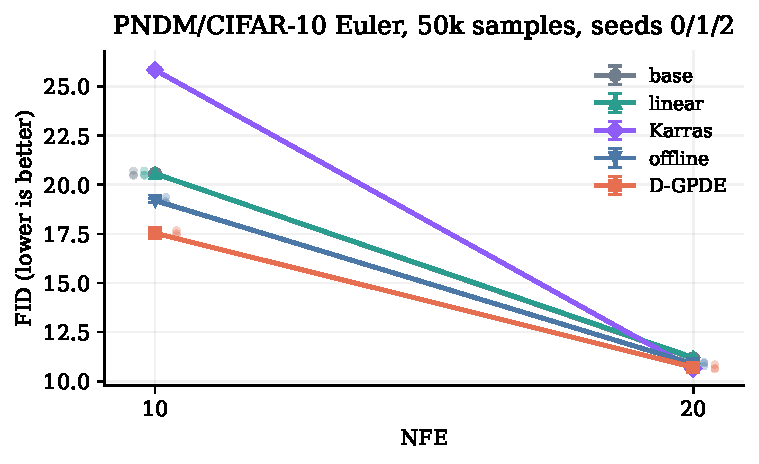
\includegraphics[width=0.68\linewidth]{figures/cifar10_pndm_euler_50k_fid_seeds0_1_2.pdf}
  \caption{PNDM/CIFAR-10 50k FID for model
  \texttt{pndm\_model\_ddim\_cifar10}, Euler solver, base, native-coordinate
  linear, fixed Karras/EDM-style, authorized project-owned offline-proxy, and
  our schedules, NFE 10 and 20, seeds 0, 1, and 2, final generation
  metric FID where lower is better. Error bars show standard error.}
  \label{fig:cifar10-pndm-euler-50k-seeds0-1-2}
\end{figure}

Figure~\ref{fig:cifar10-pndm-euler-schedule-profile-nfe20} shows the NFE-20
schedule profiles for the seed-0 calibration artifact used in the table. The
base and native-linear start grids overlap in this backend. Karras shifts more
steps toward the low-noise end, while ours redistributes start timesteps
toward the regions selected by the defect monitor.

\begin{figure}[t]
  \centering
  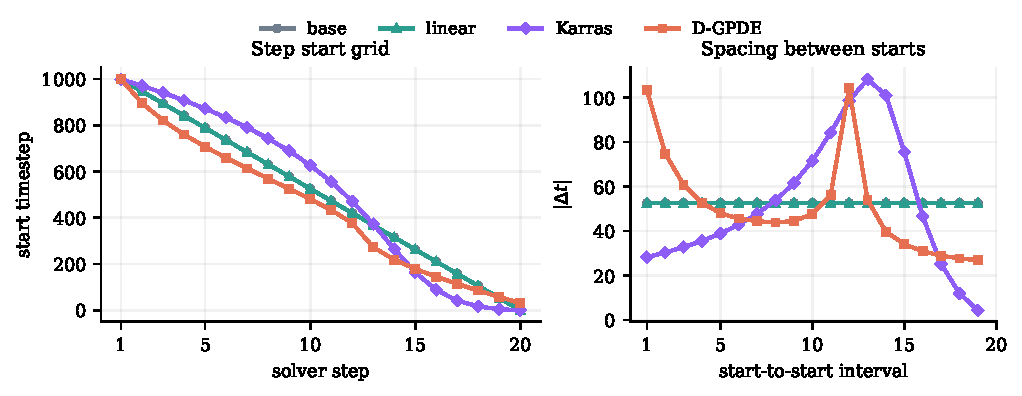
\includegraphics[width=0.78\linewidth]{figures/cifar10_pndm_euler_nfe20_schedule_profile_seed0.pdf}
  \caption{PNDM/CIFAR-10 Euler NFE-20 schedule profile for
  \texttt{pndm\_model\_ddim\_cifar10}, seed 0. The left panel shows solver-step
  start timesteps for base, native-coordinate linear, Karras/EDM-style, and
  our schedules. The right panel shows spacing between consecutive start
  timesteps. This is a schedule diagnostic, not an additional image-quality
  metric.}
  \label{fig:cifar10-pndm-euler-schedule-profile-nfe20}
\end{figure}

\begin{table}[t]
  \centering
  \caption{Actual seed-0 schedule reuse for PNDM/CIFAR-10 with
  \texttt{pndm\_model\_ddim\_cifar10}, Euler solver, NFE 10 and 20,
  seeds 1 and 2, and 50k generated images per seed. FID is
  lower-is-better. The reuse gap is seed-0-reuse FID minus seed-specific
  FID for our schedule. For these rows the continuous schedules differ by
  less than 0.002 timestep units and round to the same integer
  PNDM Euler execution grids.}
  \label{tab:cifar10-pndm-euler-50k-reuse-seed0-schedule}
  \begin{tabular}{rrrrr}
    \toprule
    NFE & base & per-seed ours & reused ours & reuse gap \\
    \midrule
    10 & 20.49 $\pm$ 0.02 & 17.47 $\pm$ 0.05 & 17.47 $\pm$ 0.05 & 0.000 $\pm$ 0.000 \\
    20 & 11.10 $\pm$ 0.02 & 10.64 $\pm$ 0.02 & 10.64 $\pm$ 0.02 & 0.000 $\pm$ 0.000 \\
    \bottomrule
  \end{tabular}
\end{table}


Table~\ref{tab:cifar10-pndm-euler-50k-reuse-seed0-schedule} reports an actual
generation reuse check: the seed-0 schedule bundle was loaded for
seeds 1 and 2, and FID was recomputed from 50k generated images per seed. In
this PNDM Euler backend, the continuous seed-specific schedules differ from the
seed-0 schedule by less than 0.002 timestep units. They round to the same
integer execution timesteps, so the reuse check verifies no execution-level FID
penalty for this configuration. It does not establish transfer across models,
solvers, prompt distributions, or CFG conditions.

The cleaned metric rows, copied schedules, linear and Karras metadata,
authorized offline metric rows, and oracle-reuse cost and reuse-validation
tables are stored under \texttt{paper/results/cifar10\_50k/}. The paper-facing
archive omits authorized offline numeric schedule bundles.
The source output roots are
\texttt{outputs/gpde\_pndm\_cifar10\_50k\_nfe10\_20\_*} and
\texttt{outputs/gpde\_pndm\_cifar10\_50k\_linear\_baseline\_seeds0\_1\_2/}
and
\texttt{outputs/gpde\_pndm\_cifar10\_50k\_karras\_baseline\_seeds0\_1\_2/}
and
\texttt{outputs/gpde\_pndm\_cifar10\_authorized\_offline/};
the actual reuse run lives under
\texttt{outputs/gpde\_pndm\_cifar10\_50k\_reuse\_seed0\_schedule\_seeds1\_2/}.

\section{Matched text-to-image CFG sweeps}

The text-to-image runs evaluate latent-diffusion models
\citep{rombach2022ldm} with the Diffusers Euler solver, NFE 10, seeds 0, 1,
and 2, and 50 prompts from \texttt{diffusers\_ablation\_prompts}. Each base,
published AYS \citep{sabour2024ays}, and our row is matched by prompt, seed,
model, solver, NFE, and guidance scale. The metrics are CLIPScore
\citep{hessel2022clipscore,radford2021clip} and ImageReward
\citep{xu2023imagereward}, where higher is better.

\subsection{Stable Diffusion 1.5}

The SD1.5 sweep uses guidance scales 5.0, 7.5, and 10.0. It retains the
largest text-to-image calibration setting in this draft, with 9 calibrated
schedules and 1350 scored images.

\begin{figure}[t]
  \centering
  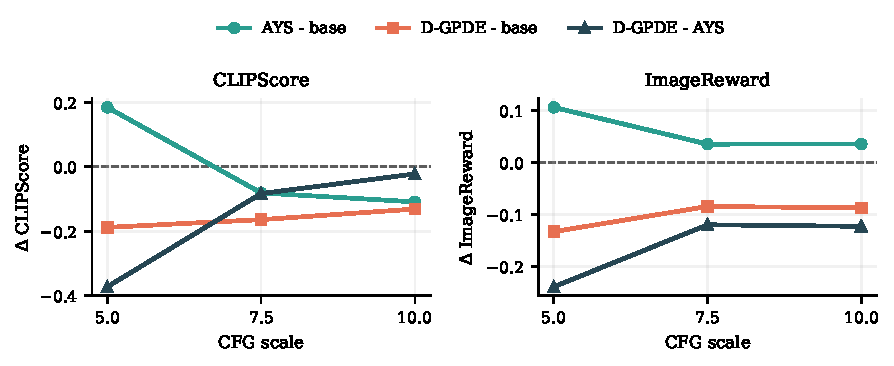
\includegraphics[width=0.86\linewidth]{figures/sd15_euler_nfe10_cfg_sweep_pairwise.pdf}
  \caption{Matched SD1.5 text-to-image pairwise mean deltas for model
  \texttt{stable\_diffusion\_15}, Diffusers Euler solver, NFE 10, guidance
  scales 5.0, 7.5, and 10.0, schedules base, AYS, and ours, seeds 0--2,
  and 50 prompts per seed from \texttt{diffusers\_ablation\_prompts}. Deltas
  are computed over 150 matched prompt/seed pairs per guidance scale. CLIPScore
  and ImageReward are higher-is-better.}
  \label{fig:sd15-euler-nfe10-cfg-sweep-pairwise}
\end{figure}

\begin{table}[t]
  \centering
  \caption{SD1.5 text-to-image matched CFG sweep with Euler solver,
  NFE 10, seeds 0--2, and 50 prompts from
  \texttt{diffusers\_ablation\_prompts}. Rows report pairwise mean
  deltas and win rates over 150 matched prompt/seed pairs. CLIPScore
  and ImageReward are higher-is-better.}
  \label{tab:sd15-euler-nfe10-cfg-sweep-pairwise}
  \begin{tabular}{llrrrr}
    \toprule
    CFG & comparison & $\Delta$CLIP & CLIP win (\%) & $\Delta$IR & IR win (\%) \\
    \midrule
    5 & AYS - base & +0.18 & 53.3 & +0.106 & 66.0 \\
    5 & ours - base & -0.19 & 42.7 & -0.133 & 33.3 \\
    5 & ours - AYS & -0.37 & 41.3 & -0.239 & 26.7 \\
    7.5 & AYS - base & -0.08 & 51.3 & +0.035 & 57.3 \\
    7.5 & ours - base & -0.16 & 45.3 & -0.084 & 46.0 \\
    7.5 & ours - AYS & -0.08 & 47.3 & -0.120 & 38.7 \\
    10 & AYS - base & -0.11 & 46.0 & +0.035 & 54.0 \\
    10 & ours - base & -0.13 & 41.3 & -0.087 & 40.7 \\
    10 & ours - AYS & -0.02 & 48.0 & -0.123 & 37.3 \\
    \bottomrule
  \end{tabular}
\end{table}


\subsection{SDXL}

The SDXL sweep \citep{podell2023sdxl} uses guidance scales 5.0 and 7.5. It
uses a lighter calibration configuration than SD1.5: one prompt per batch, four
calibration batches, 64 reference steps, a 65-node reference grid, and a
128-node candidate grid. This choice keeps the run within the minimum
validation budget while preserving the matched base/AYS/ours comparison
across three seeds.

\begin{figure}[t]
  \centering
  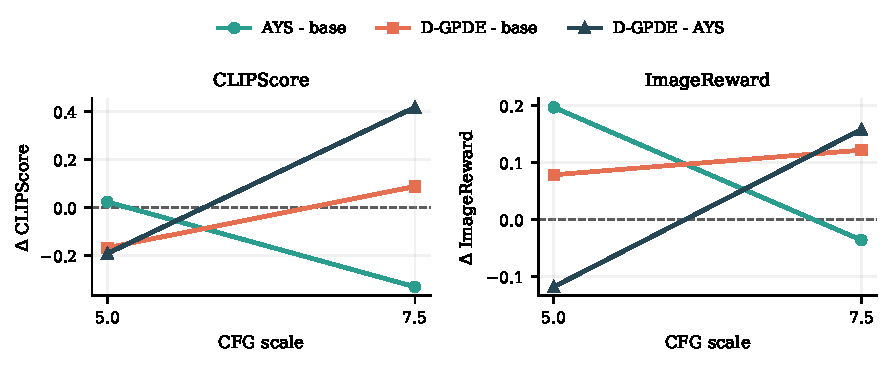
\includegraphics[width=0.86\linewidth]{figures/sdxl_euler_nfe10_cfg_sweep_pairwise.pdf}
  \caption{Matched SDXL text-to-image pairwise mean deltas for model
  \texttt{sdxl}, Diffusers Euler solver, NFE 10, guidance scales 5.0 and 7.5,
  schedules base, AYS, and ours, seeds 0--2, and 50 prompts per seed from
  \texttt{diffusers\_ablation\_prompts}. Deltas are computed over 150 matched
  prompt/seed pairs per guidance scale. CLIPScore and ImageReward are
  higher-is-better.}
  \label{fig:sdxl-euler-nfe10-cfg-sweep-pairwise}
\end{figure}

\begin{table}[t]
  \centering
  \caption{SDXL text-to-image matched CFG sweep with Euler solver,
  NFE 10, seeds 0--2, and 50 prompts from
  \texttt{diffusers\_ablation\_prompts}. Rows report pairwise mean
  deltas and win rates over 150 matched prompt/seed pairs. CLIPScore
  and ImageReward are higher-is-better.}
  \label{tab:sdxl-euler-nfe10-cfg-sweep-pairwise}
  \begin{tabular}{llrrrr}
    \toprule
    CFG & comparison & $\Delta$CLIP & CLIP win (\%) & $\Delta$IR & IR win (\%) \\
    \midrule
    5 & AYS - base & +0.02 & 46.0 & +0.197 & 66.0 \\
    5 & ours - base & -0.17 & 43.3 & +0.079 & 52.7 \\
    5 & ours - AYS & -0.19 & 48.0 & -0.119 & 35.3 \\
    7.5 & AYS - base & -0.33 & 44.7 & -0.036 & 49.3 \\
    7.5 & ours - base & +0.09 & 46.7 & +0.122 & 54.7 \\
    7.5 & ours - AYS & +0.42 & 58.0 & +0.158 & 52.7 \\
    \bottomrule
  \end{tabular}
\end{table}


The SDXL result is condition-dependent. At CFG 5.0, our schedule improves
ImageReward over base by 0.079 but trails AYS by 0.119. At CFG 7.5, it improves
the mean CLIPScore and ImageReward deltas over both base and AYS. This pattern
supports condition-aware evaluation coverage and keeps the text-to-image claim
bounded to matched automated metrics.

\subsection{SD1.5 reuse and schedule diagnostics}

\begin{table}[t]
  \centering
  \caption{Actual SD1.5 schedule reuse check. We reuse a single
  our schedule calibrated at CFG 7.5, seed 0 for CFG 5.0, 7.5,
  and 10.0, seeds 0--2, and 50 prompts per seed. Rows report matched prompt/seed
  deltas for reuse minus the CFG- and seed-specific schedule.
  Higher is better for both metrics.}
  \label{tab:sd15-euler-nfe10-reuse-cfg7p5-seed0}
  \begin{tabular}{rrrrr}
    \toprule
    CFG & $\Delta$ CLIP & CLIP win (\%) & $\Delta$ ImageReward & IR win (\%) \\
    \midrule
    5 & -0.10 & 46.7 & +0.006 & 50.7 \\
    7.5 & -0.05 & 28.0 & +0.003 & 31.3 \\
    10 & -0.00 & 48.7 & +0.034 & 53.3 \\
    \bottomrule
  \end{tabular}
\end{table}


Table~\ref{tab:sd15-euler-nfe10-reuse-cfg7p5-seed0} reports a second actual
reuse check. We reuse the CFG 7.5, seed-0 schedule for CFG 5.0, 7.5,
and 10.0, seeds 0--2, with the same 50 prompts. Reuse stays near the CFG- and
seed-specific rows on ImageReward, with matched deltas from +0.003
to +0.034, but loses CLIPScore by up to 0.10. Against base and AYS, reuse
remains negative on both automated metrics in the pairwise summaries. The
result broadens reuse evidence while preserving the text-to-image conclusion as
mixed or negative.

Figure~\ref{fig:sd15-euler-nfe10-cfg7p5-schedule-profile} shows the sigma-grid
diagnostic for the CFG 7.5, seed-0 schedule bundle. Our schedule keeps
larger sigma values for more early boundaries than both base and AYS in this
representative case. This diagnostic explains allocation only; the quality
metrics below remain the evidence for the mixed result.

\begin{figure}[t]
  \centering
  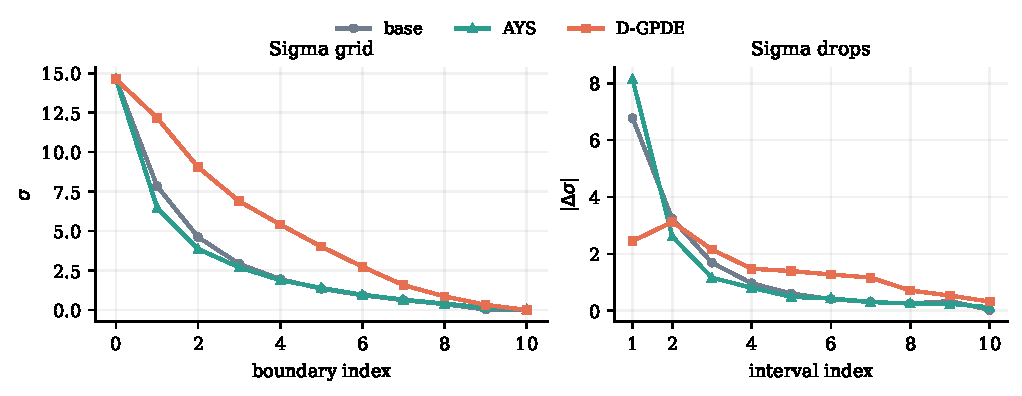
\includegraphics[width=0.82\linewidth]{figures/sd15_euler_nfe10_cfg7p5_schedule_profile_seed0.pdf}
  \caption{Stable Diffusion 1.5 Diffusers Euler NFE-10 schedule profile for
  guidance scale 7.5 and seed 0. The left panel shows the sigma grid for base,
  published AYS, and our schedules. The right panel shows sigma drops
  between adjacent boundaries. This is a schedule diagnostic, not a perceptual
  quality metric.}
  \label{fig:sd15-euler-nfe10-cfg7p5-schedule-profile}
\end{figure}

The SD1.5 sweep is a retained mixed result. AYS improves ImageReward over base
at all three guidance scales, while ours trails base and AYS on ImageReward and
underperforms base on CLIPScore under this SD1.5/Euler/NFE-10 setup. This
evidence supports a bounded failure analysis and CFG-matched evaluation
coverage. Cleaned rows, pairwise summaries, copied schedules, and oracle-reuse
cost accounting are stored under \texttt{paper/results/t2i/}. The same
directory includes the prompt manifest and prompt-index CSV for
\texttt{diffusers\_ablation\_prompts}. The source output roots are
\texttt{outputs/gpde\_diffusers\_sd15\_nfe10\_cfg\_seed\_sweep/} and
\texttt{outputs/gpde\_diffusers\_sdxl\_nfe10\_cfg\_seed\_sweep/}.

\section{Calibration Cost Accounting}

Figure~\ref{fig:calibration-cost-vs-quality} visualizes the same cost rows as
Table~\ref{tab:calibration-cost-summary}. The x-axis is logarithmic because the
matched prompt batches are small relative to the per-guidance calibration
cost. Positive quality values favor ours; negative values favor the base
schedule under the reported metric.

\begin{figure}[t]
  \centering
  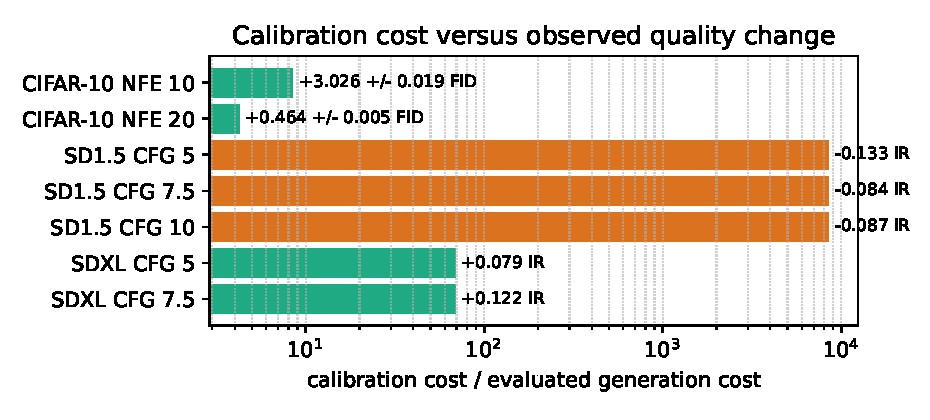
\includegraphics[width=0.9\linewidth]{figures/calibration_cost_vs_quality.pdf}
  \caption{Calibration cost versus observed quality change for current
  paper-facing runs. CIFAR-10 uses base-minus-ours FID, so positive values
  mean lower FID for ours. Text-to-image rows use ours-minus-base ImageReward,
  so negative values mean lower ImageReward for ours. Model-evaluation
  equivalents count retained calibration cost divided by the evaluated
  generation batch cost.}
  \label{fig:calibration-cost-vs-quality}
\end{figure}

The source CSV, table, and figure are generated by the aggregation script under
\texttt{paper/figures/src/}. The cleaned summary is stored under
\texttt{paper/results/cost/}.

\begin{table}[t]
  \centering
  \caption{Calibration amortization under reuse of the same schedule.
  Columns report calibration overhead divided by generation cost after
  reusing the schedule for $M$ evaluated-size batches. Break-even is the
  smallest integer $M$ for which calibration cost is no larger than
  generation cost.}
  \label{tab:calibration-amortization-summary}
  \small
  \begin{tabular}{lllrrrr}
    \toprule
    Setting & condition & quality vs. base & $M=1$ & $M=10$ & $M=100$ & break-even \\
    \midrule
    CIFAR-10 & NFE 10 & +3.026 $\pm$ 0.019 FID & 8.49$\times$ & 0.85$\times$ & 0.08$\times$ & 9 \\
    CIFAR-10 & NFE 20 & +0.464 $\pm$ 0.005 FID & 4.24$\times$ & 0.42$\times$ & 0.04$\times$ & 5 \\
    SD1.5 & CFG 5 & -0.133 IR & 8{,}487$\times$ & 848.70$\times$ & 84.87$\times$ & 8487 \\
    SD1.5 & CFG 7.5 & -0.084 IR & 8{,}487$\times$ & 848.70$\times$ & 84.87$\times$ & 8487 \\
    SD1.5 & CFG 10 & -0.087 IR & 8{,}487$\times$ & 848.70$\times$ & 84.87$\times$ & 8487 \\
    SDXL & CFG 5 & +0.079 IR & 68.62$\times$ & 6.86$\times$ & 0.69$\times$ & 69 \\
    SDXL & CFG 7.5 & +0.122 IR & 68.62$\times$ & 6.86$\times$ & 0.69$\times$ & 69 \\
    \bottomrule
  \end{tabular}
\end{table}


Table~\ref{tab:calibration-amortization-summary} shows that the current CIFAR
runs need schedule reuse across several evaluated-size batches before
calibration overhead falls below generation cost. The actual CIFAR reuse check
in Table~\ref{tab:cifar10-pndm-euler-50k-reuse-seed0-schedule} supports this
amortization only for the retained PNDM/CIFAR Euler execution grid. The SD1.5
sweep would require thousands of matched prompt batches to amortize the
calibration cost, and its observed ImageReward deltas are negative. The SDXL
sweep uses a lighter calibration setting and breaks even after 69 matched
prompt batches, but this arithmetic still needs positive reused-schedule
quality before deployment efficiency becomes supported.

\section{Broader Impacts and Asset Notes}
\label{app:responsible-assets}

Our method is a schedule-calibration method, separate from model or dataset
release. Its
positive impact, when reuse is possible, is reduced generation error at a fixed
NFE or fewer failed generations for a fixed model. Its main negative impact is
that it can also make existing generative-image systems cheaper or easier to
tune. Such systems inherit risks from their base models, including harmful
content, social bias, mis- and disinformation, impersonation, and copyright or
license misuse. The matched SD1.5 and SDXL results in this paper are reported
as automated-metric boundary cases, leaving broad text-to-image quality and
safer generation unsupported.

It also adds calibration compute. In settings where a calibrated
schedule is used only once, total compute can increase sharply. Any
deployment claim should therefore account for schedule reuse, safety filtering,
and model-license restrictions. This work uses no human subjects, private data,
or deployed system. Complete local paths for the assets below are recorded in
\texttt{configs/assets\_manifest.yaml}.

\begin{table}[t]
\centering
\caption{Current asset audit. ``Pending'' marks items that need final release
documentation before submission.}
\label{tab:asset-audit}
\scriptsize
\setlength{\tabcolsep}{3pt}
\begin{tabular}{p{0.18\linewidth}p{0.16\linewidth}p{0.30\linewidth}p{0.22\linewidth}}
\toprule
Asset & Role & Source/license status & Local record \\
\midrule
CIFAR-10 & FID benchmark and reference statistics &
Created by Krizhevsky, Nair, and Hinton; UCI lists CC BY 4.0; cite the
technical report \citep{krizhevsky2009learning}. &
CIFAR config and FID-stat asset \\
PNDM CIFAR checkpoint & Controlled sampler backend &
The official PNDM repository is Apache-2.0 and links the checkpoint/statistics
folder; cite \citet{liu2022pndm}. The release manifest records the local CIFAR
checkpoint and FID-stat hashes, but the archive should not bundle checkpoint
files without final redistribution review. &
PNDM CIFAR checkpoint asset \\
Stable Diffusion 1.5 & Text-to-image backend &
Cached model card lists \texttt{creativeml-openrail-m}. &
SD1.5 cached model card \\
SDXL & Text-to-image backend &
Cached model card and upstream terms need final author review. &
SDXL cached model record \\
AYS 10-step schedule & Published offline schedule baseline &
The official AYS quickstart lists the 10-step values; the release manifest
records local hashes. The anonymous package omits raw numeric schedule files
and retains AYS through citations, hashes, rendered figures, and metric rows. &
AYS SD1.5 and SDXL 10-step bundles \\
Diffusers & Text-to-image execution library &
Repository license is Apache-2.0. &
Diffusers vendored checkout \\
ImageReward & Text-to-image metric &
Model card and repository license are Apache-2.0. &
ImageReward checkout \\
Prompt set & Matched text-to-image prompts &
Project-local 50-prompt asset; the paper-facing manifest records hashes, while
the release license still needs final audit. &
SD prompt asset \\
\bottomrule
\end{tabular}
\end{table}

The new assets produced by this paper are experiment configs, schedule
metadata, cleaned CSVs, tables, plots, and manuscript text under
\texttt{paper/}. Draft release metadata now lives under
\texttt{paper/release/}, including an anonymized artifact manifest, license
status note, and generated-sample policy. Before release, the authors still
need to choose final licenses, finish the prompt redistribution audit, and
prepare an external anonymous archive or repository. The current release policy
omits raw AYS numeric schedule files from the anonymous package.

\section{Pilot CIFAR-10 result record}

The project retains the existing PNDM/CIFAR-10 pilot rows because they are useful
for debugging the claim-evidence loop. They are excluded from main-paper FID
claims because the run uses one seed and 5k generated images, below the
paper-grade 50k FID setting.

\begin{figure}[t]
  \centering
  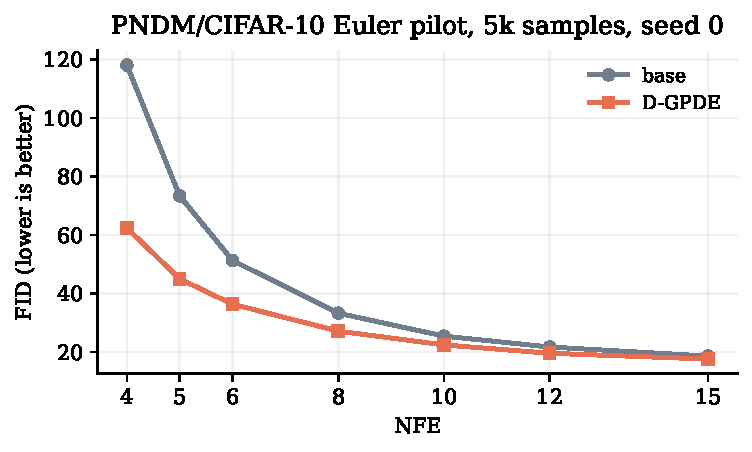
\includegraphics[width=0.78\linewidth]{figures/cifar10_pndm_euler_pilot_fid.pdf}
  \caption{PNDM/CIFAR-10 pilot FID for model
  \texttt{pndm\_model\_ddim\_cifar10}, Euler solver, base and our schedule
  schedules, NFE shown on the x-axis, seed 0, 5k generated images, final
  generation metric FID where lower is better. This is retained pilot evidence,
  not a paper-grade 50k FID result.}
  \label{fig:cifar10-pndm-euler-pilot}
\end{figure}

\begin{table}[t]
  \centering
  \caption{PNDM/CIFAR-10 FID for the Euler solver. Schedules are
  base and our schedule, NFE is listed per row, seed count is 1 seed
  (0), and FID is lower-is-better. Each row uses 5000
  generated images. This is retained pilot evidence, not paper-grade 50k FID.}
  \label{tab:cifar10-pndm-euler-pilot-fid}
  \begin{tabular}{rrrr}
    \toprule
    NFE & base FID $\downarrow$ & ours FID $\downarrow$ & FID reduction \\
    \midrule
    4 & 118.11 & 62.37 & 55.74 \\
    5 & 73.33 & 44.97 & 28.36 \\
    6 & 51.26 & 36.30 & 14.95 \\
    8 & 33.25 & 27.10 & 6.14 \\
    10 & 25.39 & 22.38 & 3.01 \\
    12 & 21.67 & 19.54 & 2.13 \\
    15 & 18.56 & 17.54 & 1.02 \\
    \bottomrule
  \end{tabular}
\end{table}


\section{Failure Analysis}
\label{app:failure-analysis}

The appendix preserves negative and mixed evidence. Retained records include
schedule mismatch cases, solver adapter failures, teacher-alignment gains with
generation-metric degradation, CFG mismatch, NaN or empty scoring checks,
unstable timestep snapping, and settings where offline baselines remain
stronger than ours.

Current retained evidence includes PNDM rho/metric ablations, two failed
project-owned offline-proxy CIFAR diagnostics, and a matched SD1.5 CFG sweep. In
the SD1.5 Euler NFE-10 sweep, ours trails base and AYS on ImageReward
across CFG 5.0, 7.5, and 10.0 and gives no CLIPScore gain. This is a concrete
negative text-to-image case.

% Auto-generated by paper/figures/src/aggregate_failure_cases.py
\begin{table}[t]
\centering
\caption{Retained failure and sensitivity cases. Positive FID deltas are worse; negative ImageReward deltas are worse.}
\label{tab:failure-cases-summary}
\scriptsize
\setlength{\tabcolsep}{3pt}
\begin{tabular}{p{0.13\linewidth}p{0.21\linewidth}p{0.16\linewidth}p{0.13\linewidth}rp{0.15\linewidth}}
\toprule
Case & Setting & Comparison & Metric & Delta & Takeaway \\
\midrule
rho=0 geometry & PNDM/CIFAR-10 Euler, NFE 10, seed 0, 5k samples & ours rho=0 - base & FID (lower better) & +30.922 & Removing the residual mix makes FID much worse than base. \\
EDM scalar metric & PNDM/CIFAR-10 Euler, NFE 10, seed 0, 5k samples & ours EDM scalar - base & FID (lower better) & +4.871 & This metric variant loses the base-schedule gain. \\
Mean aggregation & PNDM/CIFAR-10 Euler, NFE 15, seed 0, 5k samples & mean - CVaR & FID (lower better) & +0.071 & Mean aggregation remains positive but trails CVaR. \\
SD1.5 CFG 5 & SD1.5 Euler, NFE 10, 3 seeds, 50 prompts per seed & ours - base & ImageReward (higher better) & -0.133 & Matched text-to-image calibration lowers ImageReward. \\
SD1.5 CFG 7.5 & SD1.5 Euler, NFE 10, 3 seeds, 50 prompts per seed & ours - base & ImageReward (higher better) & -0.084 & Matched text-to-image calibration lowers ImageReward. \\
SD1.5 CFG 10 & SD1.5 Euler, NFE 10, 3 seeds, 50 prompts per seed & ours - base & ImageReward (higher better) & -0.087 & Matched text-to-image calibration lowers ImageReward. \\
\bottomrule
\end{tabular}
\end{table}


\begin{table}[t]
  \centering
  \caption{Retained lightweight offline-proxy CIFAR-10 baseline.
  Rows report PNDM/CIFAR-10 Euler FID, mean $\pm$ standard error over
  seeds 0, 1, and 2 with 50k generated images per seed. The
  offline-proxy schedule is a small-budget project-owned hierarchical
  coordinate-search run, not the published AYS schedule. Lower FID is
  better.}
  \label{tab:cifar10-pndm-euler-50k-offline-proxy}
  \begin{tabular}{rrrrr}
    \toprule
    NFE & base & Karras & ours & offline-proxy \\
    \midrule
    10 & 20.57 $\pm$ 0.08 & 25.84 $\pm$ 0.10 & 17.54 $\pm$ 0.08 & 41.37 $\pm$ 0.13 \\
    20 & 11.17 $\pm$ 0.07 & 10.64 $\pm$ 0.09 & 10.71 $\pm$ 0.07 & 22.36 $\pm$ 0.05 \\
    \bottomrule
  \end{tabular}
\end{table}


Table~\ref{tab:cifar10-pndm-euler-50k-offline-proxy} records a failed
small-budget project-owned offline optimization attempt for PNDM/CIFAR-10. The
optimizer used the standalone hierarchical coordinate-search exporter with 256
training images and no FID proxy early stopping. It is not the published AYS
schedule. We retain it only as negative evidence because its FID is much worse
than base, Karras, and ours at both NFE values.

Before spending 50k samples on another failed schedule, we also ran a
higher-budget offline-proxy smoke diagnostic. The exporter used 1024 training
images, seven candidates per coordinate, FID proxy early stopping for the
10-step stage, and 5k FID evaluation over seeds 0--2. It reached
$26.76 \pm 0.06$ FID at NFE 10 and $18.32 \pm 0.03$ FID at NFE 20. These
values remain far outside the competitive range, so we keep the run as failure
evidence. The paper stores the cleaned diagnostic rows and optimizer config copy
under \texttt{paper/results/failure/}.

We also logged a pre-stage-bundle default-budget attempt with 8192 training
images and 11 candidates per coordinate. Its 10-step proxy FID increased from
31.9996 to 75.8249 over four iterations after the first best value, then the
20-step refinement stage remained slow before interruption. We therefore treat
that earlier run only as feasibility evidence for default-budget cost. The
later authorized offline run uses saved NFE 10 and 20 stage bundles and appears
in the main CIFAR table. The paper stores the cleaned one-row feasibility
record under \texttt{paper/results/failure/}.

Figure~\ref{fig:sd15-failure-grid} shows the three matched SD1.5 prompt/seed
pairs with the largest ImageReward drop for ours relative to the base
Euler schedule. The paper stores the selection metadata in
\texttt{paper/results/failure/sd15\_failure\_grid\_selection.csv}.

\begin{figure}[t]
  \centering
  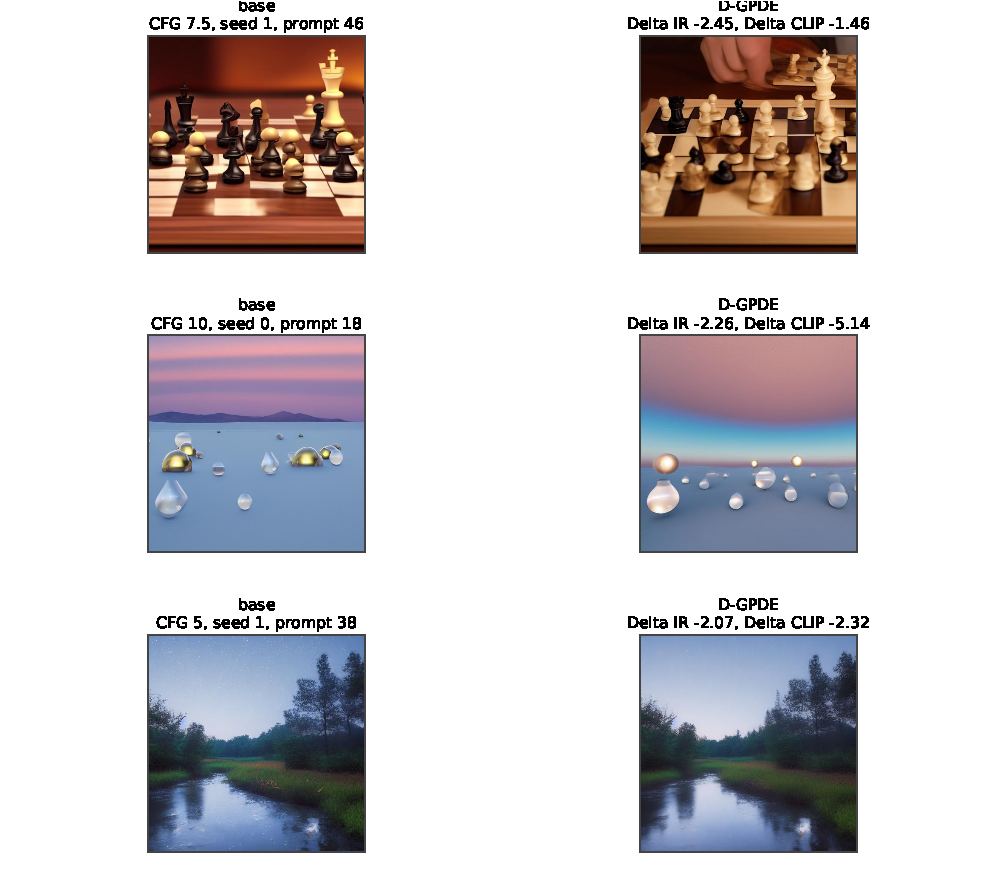
\includegraphics[width=\linewidth]{figures/sd15_failure_grid.pdf}
  \caption{Qualitative failure grid for the matched SD1.5 Euler NFE-10 CFG
  sweep. Each row compares the base schedule with ours for the same
  prompt, seed, and guidance scale. The cases are selected by the largest
  ours-minus-base ImageReward drop among retained matched samples.}
  \label{fig:sd15-failure-grid}
\end{figure}


\newpage
\input{checklist.tex}

\end{document}
